\documentclass{article}
\usepackage[margin=2.2cm]{geometry}

\usepackage{amsmath}
\usepackage{booktabs}
\usepackage{array}
\usepackage{xcolor}
\usepackage{listings}
\usepackage{tikz}
\usetikzlibrary{arrows.meta}
\usepackage[obeyspaces,spaces]{url}
\urlstyle{tt}

\definecolor{newcolor}{rgb}{0.85,0.30,0.00}   % things to be created
\definecolor{ovcolor}{gray}{0.35}               % overview
\definecolor{expcolor}{rgb}{0.12,0.28,0.62}   % explanation only, nothing to code
\newcommand{\partbanner}[4]{% colour, label, title, subtitle
  \noindent\fcolorbox{#1}{#1!8}{\parbox{\dimexpr\linewidth-2\fboxsep-2\fboxrule\relax}{%
    \textbf{\large #2: #3}\\[1mm]\small #4}}\par\bigskip}
\lstset{basicstyle=\ttfamily\footnotesize, frame=single, keepspaces=true,
        showstringspaces=false, aboveskip=6pt, belowskip=4pt,
        moredelim=[is][\color{newcolor}]{@@}{@@}}

\tikzset{
  box/.style={draw, rounded corners=2pt, minimum width=4.4cm, minimum height=0.8cm,
              align=center, font=\footnotesize, fill=black!6},
  newbox/.style={box, draw=newcolor, line width=1pt, fill=newcolor!8},
  later/.style={box, dashed, fill=white, draw=black!50, text=black!60},
  lab/.style={font=\scriptsize\itshape, text=black!70, align=left},
  flow/.style={-{Stealth[length=2mm]}, thick},
}

\title{Technical Requirements:\\ \texttt{physics}, \texttt{inversion} and \texttt{isolines}\\[1mm]
       \large UKRAINIX WATERDRONE -- analysis-app}
\author{}
\date{27 November 2026}

\begin{document}
\maketitle

\partbanner{ovcolor}{Part I}{Overview}{What is built, how the pieces connect, and the conventions
used everywhere.}

\section{Scope and conventions}

This document specifies three packages of the analysis app (inside
\path{src/analysis_app/}): \path{physics}, \path{inversion} and \path{isolines}.
\path{core} and \path{parsing} are finished and are not touched. Nothing else of
the planned app (\path{normalization}, \path{pipeline}, \path{viz}, \path{gui}) is
needed now, and nothing else should be written yet.

\paragraph{How this document is organised.} The physics \emph{explanation} and the
\emph{file creation} are kept apart on purpose:

\begin{center}\small
\begin{tabular}{@{}l l p{9.6cm}@{}}
\toprule
Part & Sections & Content \\
\midrule
\textcolor{ovcolor}{\textbf{I -- Overview}} & 1--2 &
   Scope, conventions, data flow and dependencies. \\
\textcolor{expcolor}{\textbf{II -- Physics model}} & 3 &
   \textbf{Explanation only.} Where the formulas come from, what they mean, when they
   hold. It contains no file names, function names or code, and \textbf{nothing in it is
   to be coded by itself}. \\
\textcolor{newcolor}{\textbf{III -- What to create}} & 4--9 &
   \textbf{All the work.} Files, functions, signatures, examples and acceptance checks.
   This is the only place that says what to write; it refers to formulas of Part II by
   their number. \\
\bottomrule
\end{tabular}
\end{center}

\begin{itemize}
\item \textbf{Simplicity first.} Write only what is listed in Part III. If in doubt, do
      not write it. \textbf{No tests} are written in this step.
\item \textbf{No data validation.} Assume well-formed arrays.
\item \textbf{Plain arrays in, plain arrays out.} The three packages never see a
      \path{Sample}; they take numpy arrays (Table~\ref{tab:arrays} in Section~\ref{sec:files}). Choosing
      one parameter of a \path{Sample} and dropping its empty (NaN) cells is the
      caller's job (the later \path{pipeline}); all arrays given to these packages
      are finite.
\item \textbf{Style.} Plain functions; the only class is the \path{NamedTuple}
      \path{Model}. Inputs are never modified in place. Each package's
      \path{__init__.py} re-exports its public names, and callers import from the
      package, not from its files.
\item \textbf{Units.} $x,y$: local metres (output of \path{parsing}). $z$: depth
      below the water surface in metres, positive downwards (CSV column
      \path{Z}). Parameter values $v$ in the units of the CSV.
\item \textbf{Everything is per parameter.} One call handles one CAPS parameter;
      looping over the parameters is the job of the later \path{pipeline}.
\end{itemize}



\section{Data flow, relations and dependencies}

\begin{center}
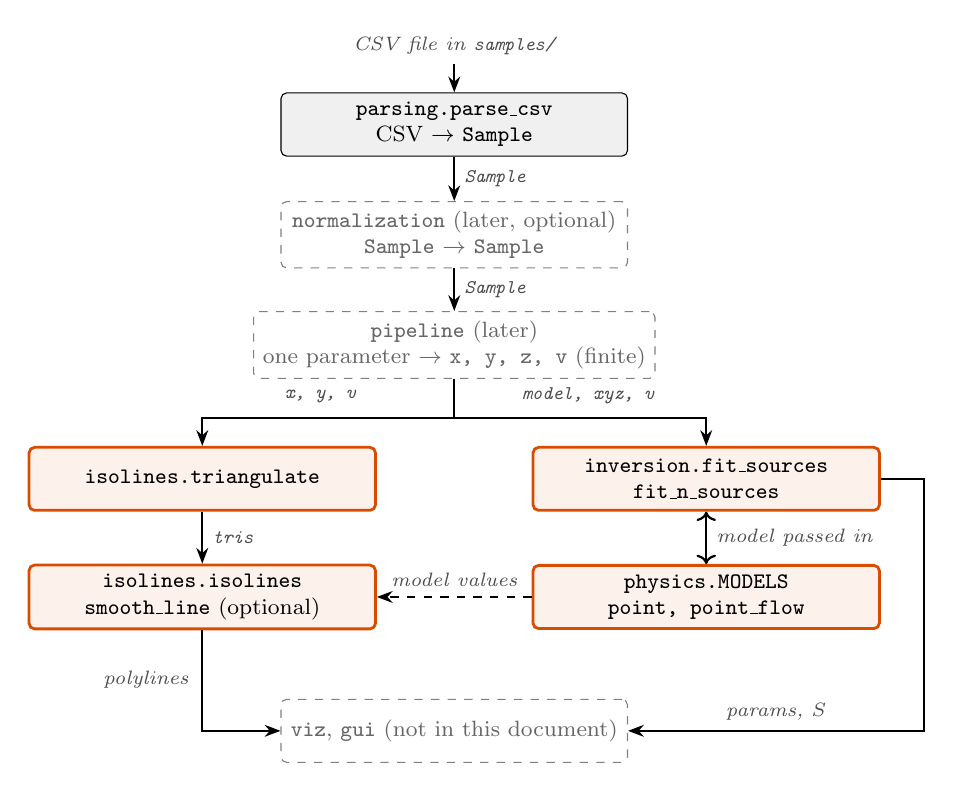
\begin{tikzpicture}[x=1cm,y=1cm]
\node[lab] (csv) at (0,0) {CSV file in \texttt{samples/}};
\node[box] (parse) at (0,-1.0) {\texttt{parsing.parse\_csv}\\ CSV $\to$ \texttt{Sample}};
\node[later] (norm) at (0,-2.4) {\texttt{normalization} (later, optional)\\ \texttt{Sample} $\to$ \texttt{Sample}};
\node[later] (pa) at (0,-3.8) {\texttt{pipeline} (later)\\ one parameter $\to$ \texttt{x, y, z, v} (finite)};
\node[newbox] (tri) at (-3.2,-5.5) {\texttt{isolines.triangulate}};
\node[newbox] (iso) at (-3.2,-7.0) {\texttt{isolines.isolines}\\ \texttt{smooth\_line} (optional)};
\node[newbox] (fit) at (3.2,-5.5) {\texttt{inversion.fit\_sources}\\ \texttt{fit\_n\_sources}};
\node[newbox] (phy) at (3.2,-7.0) {\texttt{physics.MODELS}\\ \texttt{point, point\_flow}};
\node[later] (viz) at (0,-8.7) {\texttt{viz}, \texttt{gui} (not in this document)};

\draw[flow] (csv) -- (parse);
\draw[flow] (parse) -- node[lab,right] {\texttt{Sample}} (norm);
\draw[flow] (norm) -- node[lab,right] {\texttt{Sample}} (pa);
\draw[flow] (pa.south) -- ++(0,-0.5) -| (tri.north);
\draw[flow] (pa.south) -- ++(0,-0.5) -| (fit.north);
\node[lab] at (-1.7,-4.45) {\texttt{x, y, v}};
\node[lab] at (1.7,-4.45) {\texttt{model, xyz, v}};
\draw[flow] (tri) -- node[lab,right] {\texttt{tris}} (iso);
\draw[flow,<->] (fit) -- node[lab,right] {model passed in} (phy);
\draw[flow,dashed] (phy.west) -- node[lab,above] {model values} (iso.east);
\draw[flow] (iso.south) |- (viz.west);
\node[lab,left] at (-3.25,-8.05) {polylines};
\draw[flow] (fit.east) -- ++(0.55,0) |- node[lab,above,pos=0.75] {params, $S$} (viz.east);
\end{tikzpicture}
\end{center}

\noindent Orange = written in this step. Grey = already exists. Dashed box =
later. The dashed arrow is optional and costs no code: calling \path{isolines}
with the fitted model's values instead of the measured $v$ draws the isolines
of the fitted field.

\begin{table}[!ht]
\centering\small
\begin{tabular}{@{}l l l p{3.6cm} p{3.6cm}@{}}
\toprule
Package & Imports (in app) & Used by & Takes & Returns \\
\midrule
\path{parsing}   & \path{core} & \path{pipeline} & CSV path & \path{Sample} \\
\path{physics}   & numpy only & \path{pipeline} & \path{glob}, \path{src}, $xyz$ & model values \\
\path{inversion} & none (numpy, scipy) & \path{pipeline} & model, $xyz$, $v$ & \path{glob}, \path{src}, $S$ \\
\path{isolines}  & none (numpy, scipy) & \path{pipeline}, \path{viz} & $x,y,v$, levels & polylines \\
\bottomrule
\end{tabular}
\caption{Dependencies. Nothing imports upwards.}
\end{table}

\paragraph{Rules.}
\begin{enumerate}
\item \path{physics}, \path{inversion} and \path{isolines} do not import
      \path{core}, \path{parsing} or each other. They take arrays (and, for
      \path{inversion}, a \path{Model}), so the three can be written and run in
      parallel, in any order, with made-up arrays.
\item \path{inversion} receives the model as an argument and never imports a
      particular model; the \path{pipeline} passes \path{MODELS[name]}. A model
      is chosen by name, so several models with different numbers of parameters
      live side by side (Section~\ref{sec:physics}).
\item \path{isolines} knows nothing about physics. The two branches meet only
      later, in \path{pipeline} and \path{viz}.
\item Normalization, when it exists, maps \path{Sample} $\to$ \path{Sample} before
      one parameter is cut out. Nothing in this document changes then.
\item Suggested order: \path{physics/models.py} $\to$ \path{inversion/fit.py};
      \path{isolines/triangulation.py} $\to$ \path{isolines/contours.py}
      $\to$ \path{smooth_line}.
\end{enumerate}





\clearpage
\partbanner{expcolor}{Part II}{Physics model -- explanation only}{Why the model has the form it has
(lecture T5). \textbf{Nothing in this part is to be coded as it stands:} it has no file names or
function names. Part III turns the results into code.}

\section{The physical model (lecture T5)}
\label{sec:theory}

\subsection{The field and its equation}

The three groups of water parameters -- pollutant concentration, acidity and
temperature -- are all ``an amount of something per unit volume'' carried by
particles, so they obey the same equation. Write $u(x,y,z,t)$ for that field.
Two ideas are enough: particles do not disappear (continuity), and they spread
from crowded to empty places (Fick's law):
\[
\frac{\partial u}{\partial t}+\operatorname{div}\vec j=q,
\qquad
\vec j=-D\,\operatorname{grad}u
\quad\Longrightarrow\quad
\frac{\partial u}{\partial t}=D\,\Delta u+q ,
\qquad
\Delta u=\frac{\partial^2u}{\partial x^2}+\frac{\partial^2u}{\partial y^2}+\frac{\partial^2u}{\partial z^2}.
\tag{1}
\]
After a long, steady emission nothing changes in time, $\partial u/\partial t=0$:
\[
D\,\Delta u=-q \quad(\text{Poisson, with sources}),\qquad
\Delta u=0 \quad(\text{Laplace, between the sources}).
\tag{2}
\]
This is the working equation: it contains no time, so one survey is a snapshot,
and it is linear, so solutions of different sources add up.

\begin{table}[h]
\centering\small
\begin{tabular}{@{}l p{8.4cm} l@{}}
\toprule
Symbol & Meaning & Unit \\
\midrule
$u$ & field: concentration (mg/L $=$ g/m$^3$), ion concentration, or temperature & $[u]$ \\
$u_\infty$ & background value far from all sources & $[u]$ \\
$D$ & diffusion coefficient (effective, turbulent, in a lake: $10^{-5}\dots10^{-2}$) & m$^2$/s \\
$Q_i$ & power of point source $i$ (amount emitted per second) & $[u]\,$m$^3$/s \\
$w_i=Q_i/(4\pi D)$ & strength of source $i$ & $[u]\,$m \\
$\vec r_i=(x_i,y_i,z_i)$ & position of source $i$ (depth $z_i\ge0$) & m \\
$\vec v$ & velocity of the current & m/s \\
$\vec\kappa=\vec v/(2D)$ & current relative to diffusion; $|\vec\kappa|=1/\ell$ & 1/m \\
\bottomrule
\end{tabular}
\caption{Symbols. For temperature $D$ is the thermal diffusivity
$a=\lambda/(\rho c)$ and $Q$ is the heater power divided by $\rho c$.}
\end{table}

\subsection{One source and several sources}

\paragraph{One point source.}
By symmetry $u$ depends only on the distance $r$ from the source, so the flux
through every sphere is the source power: $j(r)\cdot4\pi r^2=Q$. With
$\Delta u=0$ for $r>0$ and $u\to u_\infty$ far away this gives
\[
u(r)=u_\infty+\frac{Q}{4\pi D\,r}.
\tag{3}
\]
Check of units: $[Q]/([D][r])=(\mathrm{g/s})/((\mathrm{m^2/s})\,\mathrm m)=\mathrm{g/m^3}$.
The same equation and solution describe the electric potential
($u\leftrightarrow\varphi$, $D\leftrightarrow\varepsilon_0$, $Q\leftrightarrow q$):
this is the form $Q_i/(4\pi\varepsilon_0|\vec r-\vec r_i|)$ of the handwritten
note, and $\sigma$ (conductivity) plays the same role for an electric current.

\paragraph{Several sources.} Equation~(2) is linear, so the sources add up. With
sources at $\vec r_i$ and a sample at $\vec r_k=(x_k,y_k,z_k)$ the model field is
\begin{equation}
u_T(\vec r_k)=u_\infty+\sum_{i=1}^{N}\frac{w_i}{r_{ki}},\qquad
r_{ki}=\sqrt{(x_k-x_i)^2+(y_k-y_i)^2+(z_k-z_i)^2},\qquad w_i=\frac{Q_i}{4\pi D}\ge0 .
\tag{4}
\end{equation}
Sample and source depths are measured the same way (metres below the surface,
positive down), and $r$ is the three-dimensional distance. This is the field used
throughout, and exactly the field used to generate the synthetic phase-1 samples
(there $u_\infty=0$). The number of sources $N$ is a property of the lake and is
\emph{not known in advance}.

\subsection{What the measurements can and cannot determine}

Equation~(3) contains $Q$ and $D$ only as the ratio $w=Q/(4\pi D)$, so measurements
determine $w_i$, $u_\infty$ and the positions, \emph{never $Q_i$ and $D$ separately}.
No physical constants therefore appear in the working formulas: all of them are
inside $w_i$. $Q_i$ follows only if $D$ is known from elsewhere, and vice versa.

\subsection{The criterion for the best fit}

For measured values $u_e(\vec r_k)$ at $K$ points the misfit is
\[
S=\sum_{k=1}^{K}\bigl(u_T(\vec r_k)-u_e(\vec r_k)\bigr)^2 .
\tag{5}
\]
The best choice of $u_\infty$, positions and strengths -- and, if it is not known, of
the number of sources $N$ -- is the one with the smallest $S$ (the minimum gives
$u_T^{\min}$ of the handwritten note). A true source that is missing from the model
raises $S$ strongly; an extra one on noisy data lowers it only slightly.

\subsection{Where the model holds}

\begin{itemize}
\item \textbf{Input is a concentration-like quantity.} For acidity the field is
      $[\mathrm H^+]=10^{-\mathrm{pH}}$, not the pH itself (pH is a logarithm and
      logarithms do not add); the conversion has to be done before such data are
      compared with the model.
\item Stationary state; homogeneous, isotropic water with one constant $D$;
      dilute impurity; no reaction, decay or settling; unbounded water. A source
      \emph{on} the surface emits into a half-space, $j\cdot2\pi r^2=Q$, and
      gives the same formula with $w=Q/(2\pi D)$ (twice the concentration): only
      the meaning of $w$ changes. Reflections of deeper sources at surface,
      bottom and shore are not modelled.
\item Far field: the formula is meant for distances much larger than the source
      size ($u\to\infty$ at $r\to0$ is a sign that the point model fails there)
      and not much larger than the depth $H$ (beyond that the spreading becomes
      horizontal and the $1/r$ law turns into a logarithmic one).
\end{itemize}

\subsection{A source in a current}

A uniform current $\vec v$ adds transport by the water, $\vec j=u\vec v-D\operatorname{grad}u$:
\[
\frac{\partial u}{\partial t}+\vec v\cdot\operatorname{grad}u=D\,\Delta u+q .
\tag{6}
\]
For a steady point source the solution is
\[
u=u_\infty+\frac{Q}{4\pi D\,r}\exp\!\Bigl[-\frac{r}{\ell}\,(1-\cos\theta)\Bigr],\qquad
\ell=\frac{2D}{v},
\]
where $\theta$ is the angle between the current and the direction from the source
to the sample ($\theta=0$ downstream, the factor is 1; upstream it is $e^{-2r/\ell}$).
Since $r\cos\theta=\hat v\cdot(\vec r_k-\vec r_i)$ and $1/\ell=|\vec\kappa|$, the field
of $N$ sources in a horizontal current $\vec\kappa=(\kappa_x,\kappa_y,0)$ is
\begin{equation}
u_T(\vec r_k)=u_\infty+\sum_{i=1}^{N}\frac{w_i}{r_{ki}}
\exp\!\bigl[\kappa_x(x_k-x_i)+\kappa_y(y_k-y_i)-|\vec\kappa|\,r_{ki}\bigr].
\tag{7}
\end{equation}
The current is the same for all sources, so $\kappa_x,\kappa_y$ are properties of the
lake, not of a source; $\vec\kappa=0$ gives equation~(4). The current matters only at
distances $r$ of the order of $\ell$ or more (for $D=10^{-2}$~m$^2$/s and $v=2$~mm/s: $\ell=10$~m).
Again only the ratios $w=Q/(4\pi D)$ and $\kappa=v/(2D)$ are determined.

\subsection{Extended sources (explained, not used)}

A real source has a size, and its far field is a series
$u-u_\infty=\frac1{4\pi D}\bigl[\frac{m_0}{r}+\frac{m_1\cos\theta}{r^2}+
\frac{m_2(3\cos^2\theta-1)/2}{r^3}+\dots\bigr]$ (point, dipole, quadrupole, \dots;
$m_0=Q$). These terms matter only at $r\sim a$ (source size), and each adds one more
parameter per source. In a numerical test (two sources with a vertical dipole term,
geometry of the synthetic lakes) the fit reached a small misfit but with the source
depth wrong by 19~m and $m_1$ wrong by $10^4$: for surveys at $z=1\dots10$~m the dipole
term is almost degenerate with depth and strength. These corrections are therefore
\emph{not used}. (The lecture's $z$ axis points up and ours points down, so $\cos\theta$ in
the dipole term changes sign; equation~(7) is for a horizontal current and is not affected.)

\subsection{In short}

\begin{center}
\fcolorbox{expcolor}{expcolor!8}{\parbox{0.93\linewidth}{\small
\textbf{The working model.}
\begin{itemize}\itemsep=0pt
\item Field of $N$ point sources: equation~(4); in a uniform horizontal current:
      equation~(7).
\item Unknowns: the background $u_\infty$, for each source its position and strength
      $w_i$, and (with a current) $\kappa_x,\kappa_y$. $N$ itself is also unknown.
\item Determined by data: $w=Q/(4\pi D)$ and $\kappa=v/(2D)$ -- never $Q$, $D$, $v$ alone.
\item Criterion: least squares, equation~(5).
\item Valid for: a stationary state, uniform water, distances well above the source
      size; the input is a concentration-like quantity.
\end{itemize}}}
\end{center}

\clearpage
\partbanner{newcolor}{Part III}{What to create}{Files, functions, signatures, examples and acceptance
checks. Everything to be written is specified here and only here. Formula numbers refer to
Part II.}

\section{Files to create and libraries to use}
\label{sec:files}

Files shown in \textcolor{newcolor}{\textbf{orange}} are to be created; marked
\texttt{[new]}. \path{physics/} is not in the committed tree (git does not store
empty folders), so it has to be created.

\begin{lstlisting}
src/analysis_app/
|-- physics/
|   |-- @@__init__.py@@              [new]
|   \-- @@models.py@@                [new]
|-- inversion/
|   |-- @@__init__.py@@              [new]
|   \-- @@fit.py@@                   [new]
\-- isolines/
    |-- @@__init__.py@@              [new]
    |-- @@triangulation.py@@         [new]
    \-- @@contours.py@@              [new]
\end{lstlisting}

\paragraph{Libraries to use.}
\begin{itemize}
\item \path{numpy} -- all arrays, all vectorised arithmetic (no Python loops over
      samples in \path{physics} and \path{inversion});
\item \path{scipy.optimize.least_squares} -- the minimisation in \path{inversion};
\item \path{scipy.spatial.Delaunay} -- the triangulation;
\item \path{scipy.interpolate.splprep}, \path{splev} -- the optional smoothing;
\item standard library -- \path{typing} for \path{NamedTuple} and \path{Callable}.
\end{itemize}
\noindent \path{scipy} is a new dependency of the project; add it to the project's
list of dependencies.

\paragraph{Arrays that cross package boundaries.} All three packages exchange only the arrays of Table~\ref{tab:arrays}.

\begin{table}[h]
\centering\small
\begin{tabular}{@{}l l p{9.2cm}@{}}
\toprule
Name & Shape & Meaning \\
\midrule
\path{x, y, z, v} & $(n,)$ & Sample coordinates (m), depth (m, positive down) and
                    parameter values; all finite. \\
\path{xyz}        & $(n,3)$ & \path{np.column_stack([x, y, z])}. \\
\path{glob}       & $(G,)$ & Global parameters of a model (the same for all sources),
                    e.g.\ the background $u_\infty$. $G$ depends on the model. \\
\path{src}        & $(N,P)$ & One row per source. Columns: $x_i, y_i, z_i$, then the
                    other per-source parameters of the model (strength $w_i$, \dots);
                    $P$ depends on the model. The number of sources $N$ is \emph{not
                    known in advance}: it is found by \path{inversion}. \\
\path{tris}       & $(m,3)$ int & Vertex indices into \path{x, y, v}. \\
\path{levels}     & $(L,)$ & Values at which isolines are wanted. \\
polyline          & $(k,2)$ & Points $(x,y)$ in order; for a closed isoline the
                    first point is repeated at the end. \\
\bottomrule
\end{tabular}
\caption{Arrays that cross package boundaries.}
\label{tab:arrays}
\end{table}

\section{What is assumed to exist}

\begin{itemize}
\item \path{analysis_app.parsing}: \path{parse_csv(path, ref_origin=None)}
      returning a \path{Sample} (fields \path{x, y, depth, values}), and
      \path{latlon_to_xy}. The three packages above do not import it; it is how
      the data and the true sources for the checks in Section~\ref{sec:done} are
      obtained.
\item Test data in the repository-level \path{samples/} folder:
      \path{phase1_synthetic/reduced/*.csv} (five lakes generated with the field of
      equation~(4), background $u_\infty=0$) with the true sources in
      \path{phase1_synthetic/config/*.txt} (lines
      \path{ORIGIN PARAM lat lon depth weight}), and the real Utah Lake files in
      \path{phase2_real/reduced/}.
\end{itemize}

\section{Package \texttt{physics}}
\label{sec:physics}

\subsection{From the explanation to the code}

Part II is explanation; this table is the only link between it and the code.

\begin{table}[h]
\centering\small
\begin{tabular}{@{}l l p{6.6cm}@{}}
\toprule
In Part II & In the code & Note \\
\midrule
$u_e$, measured values & \path{v} & argument of the \path{inversion} functions \\
$u_\infty$ & \path{glob}, name \path{u_inf} & first global parameter of every model \\
$x_i,y_i,z_i$ & \path{src} columns 0, 1, 2 & names \path{x, y, z} \\
$w_i$ & \path{src} column 3 & name \path{w} \\
$\kappa_x,\kappa_y$ & \path{glob}, names \path{kx, ky} & only in \path{"point_flow"} \\
$D$, $Q_i$, $\vec v$ & -- & do not appear: they are inside $w_i$ and $\kappa$ \\
equation (4) & \path{MODELS["point"]} & \\
equation (7) & \path{MODELS["point_flow"]} & \\
equation (5) & residual in \path{inversion/fit.py} & \path{model.func(...) - v} \\
\bottomrule
\end{tabular}
\end{table}

\noindent \textbf{Not to be coded}, although explained in Part II: the surface-source factor 2
(only the meaning of $w$ changes), reflections, time dependence, the source size
corrections $m_1,m_2,\dots$. The interface below would allow the last ones (more
per-source columns, one more \path{setup} entry), but Section~\ref{sec:theory}
explains why they are not used.

\subsection{\texttt{physics/models.py}}
\label{sec:model}

A model is described by a \path{NamedTuple} so that the inversion can handle any
number of parameters without knowing the formula:

\begin{lstlisting}
class Model(NamedTuple):
    func:       Callable   # func(glob, src, xyz) -> (n,)
    glob_names: tuple      # names of the G global parameters
    src_names:  tuple      # names of the P per-source parameters; always starts "x","y","z"
    setup:      Callable   # setup(E, v) -> (glob_spec, src_spec)
\end{lstlisting}

\begin{itemize}
\item \path{func(glob, src, xyz)}: \path{glob} $(G,)$, \path{src} $(N,P)$,
      \path{xyz} $(n,3)$ $\to$ $(n,)$ array of model values. Vectorised by
      broadcasting to shape $(n,N,3)$, no loops. Distance zero is not handled.
      $G=\texttt{len(glob\_names)}$ and $P=\texttt{len(src\_names)}$ may differ
      between models; $N$ is whatever the caller passes.
\item \path{setup(E, v)}: tells the inversion where to start and how far the
      parameters may go. \path{E} is the larger of the ranges of $x$ and $y$
      (metres), \path{v} the measured values. It returns
      \path{(glob_spec, src_spec)}: two lists of tuples
      \path{(start, lower, upper, scale)}, one tuple per name in \path{glob_names}
      and one per name in \path{src_names[3:]} (the inversion handles $x,y,z$
      itself). \path{scale} is a typical size of the parameter.
\item \path{MODELS}: dictionary name $\to$ \path{Model}, with the two models below (equations (4) and (7)).
      Private helpers (\path{_delta} for the differences and distances,
      one \path{_setup_...} per model) are allowed.
\end{itemize}

\begin{table}[h]
\centering\small
\begin{tabular}{@{}l l l l l@{}}
\toprule
Name & \path{glob_names} & \path{src_names} & Unknowns for $N$ sources & Equation \\
\midrule
\path{"point"}      & \path{u_inf} & \path{x y z w} & $1+4N$ & (4) \\
\path{"point_flow"} & \path{u_inf kx ky} & \path{x y z w} & $3+4N$ & (7) \\
\bottomrule
\end{tabular}
\end{table}

\begin{table}[h]
\centering\small
\begin{tabular}{@{}l l l l l@{}}
\toprule
Parameter & start & lower & upper & scale \\
\midrule
\path{u_inf} & $\min v$ & $-\infty$ & $+\infty$ & $\operatorname{range}(v)$ \\
\path{w}     & $0.05\,E\cdot\operatorname{range}(v)$ & 0 & $+\infty$ & the start value \\
\path{kx, ky} & 0 & $-10$ & $+10$ & $10/E$ \\
\bottomrule
\end{tabular}
\caption{Output of \texttt{setup}. $\operatorname{range}(v)=\max v-\min v$. Do not
bound $u_\infty$ from above by $\min v$: noise pushes some values below the true
background and the fit then sticks at the bound.}
\end{table}

Adding a model later (different current, a source with a size, \dots) means: one
function, one \path{setup} function, one dictionary entry. Nothing in
\path{inversion} changes.

\begin{lstlisting}
>>> m = MODELS["point"]
>>> src = np.array([[0., 0., 10., 100.]])                   # x, y, z, w
>>> m.func(np.array([2.0]), src, np.array([[0., 0., 0.], [10., 0., 0.]]))
array([12.   ,  9.071])                       # 2 + 100/10  and  2 + 100/sqrt(200)
>>> src2 = np.array([[0., 0., 10., 100.], [30., 0., 10., 50.]])
>>> m.func(np.array([0.0]), src2, np.array([[0., 0., 0.]]))
array([11.581])                               # 100/10 + 50/sqrt(1000)
>>> f = MODELS["point_flow"]                      # glob = u_inf, kx, ky
>>> f.func(np.array([0., 0.01, 0.]), src, np.array([[10., 0., 0.], [-10., 0., 0.]]))
array([6.784, 5.554])                         # downstream value is larger
>>> f.func(np.array([0., 0., 0.]), src, np.array([[10., 0., 0.]]))
array([7.071])                                # kappa = 0: same as "point"
\end{lstlisting}


\section{Package \texttt{inversion}}

\subsection{\texttt{inversion/fit.py}}

Finds the parameters that minimise the misfit~(5): the $G$ global parameters and
the $N$ rows of \path{src}, i.e.\ $G+NP$ unknowns, for a given \path{Model}. The
number of sources is \emph{not known in advance}, so there are two functions:
\path{fit_n_sources} for a given $N$, and \path{fit_sources}, which finds $N$.

\begin{lstlisting}
fit_n_sources(model, xyz, v, n_sources, n_starts=5, seed=0, max_nfev=100)
    -> (glob, src, S)
fit_sources(model, xyz, v, n_max=6, n_starts=5, seed=0, gain=0.5, max_points=3000)
    -> (glob, src, S_list)
\end{lstlisting}
\begin{itemize}
\item \path{fit_n_sources}: \path{glob} $(G,)$, \path{src} $(N,P)$ with rows
      sorted by the column \path{w} (index~3) ascending, so the order is
      reproducible; $S$ is a Python float, $S=\sum(\text{residual})^2$.
\item \path{fit_sources}: the number of sources is \path{len(src)};
      \path{S_list[k]} is $S$ for $k+1$ sources, the last entry belongs to the
      returned sources.
\end{itemize}

\paragraph{\texttt{fit\_n\_sources}.}
\begin{itemize}
\item Put all unknowns in one vector $p=[\texttt{glob},\ \texttt{src}[0],\
      \texttt{src}[1],\dots]$ and use \path{scipy.optimize.least_squares} on the
      residual vector \path{model.func(p[:G], p[G:].reshape(-1, P), xyz) - v}.
\item $E=\max(\operatorname{range}x,\operatorname{range}y)$, $z_0=0.05\,E$.
      Bounds and scales of $x,y$: inside the bounding box of the samples, scale
      $E/20$. Of $z$: $0\le z\le E$, scale $z_0$. Everything else (global and the
      other per-source parameters) comes from \path{model.setup(E, v)}. Pass the
      scales as \path{x_scale}: the unknowns differ by orders of magnitude and the
      fit fails without it.
\item Start: choose \path{n_sources} random samples (\path{numpy.random.default_rng(seed)});
      their $x,y$ are the source positions, $z=z_0$, all other parameters at their
      \path{start}. Run \path{n_starts} such starts with \path{max_nfev} iterations
      each and keep the one with the lowest cost.
\item Why several starts: one start finds the global minimum in 8 of 10 cases (different seeds)
      on the four-source lake, five starts in 10 of 10; a failed start is easy to
      see, its $S$ is orders of magnitude larger. Why \path{max_nfev}: an
      over-parameterised fit (more sources than exist) wanders along flat valleys;
      a single search took 20 to 75~s without the cap.
\end{itemize}

\paragraph{\texttt{fit\_sources}: how $N$ is found.}
\begin{enumerate}
\item Thin the data: \path{step = max(1, len(v) // max_points)}, use
      \path{xyz[::step]} and \path{v[::step]} for all fits below. The surveys have
      thousands of nearly identical neighbours; with all points one search
      took 20--75~s, thinned 1--3~s, with the same sources to better than 0.01~m.
      Pass \path{max_points=len(v)} to use everything.
\item For $N=1,2,\dots,\texttt{n\_max}$ call \path{fit_n_sources} and store $S_N$.
      Stop as soon as one of two things happens:
      \begin{itemize}
      \item $S_N\le10^{-8}\sum_k(v_k-\bar v)^2$: the fit is perfect (noise-free
            synthetic data), nothing can be improved; keep $N$ sources;
      \item $N\ge2$ and $S_N>\texttt{gain}\cdot S_{N-1}$: the extra source did not
            at least halve the misfit, so $N-1$ sources are enough; drop the last
            fit and keep $N-1$.
      \end{itemize}
      If the loop ends at \path{n_max}, return that fit.
\item Return \path{glob} and \path{src} of the kept fit and the list of its $S$ values.
\end{enumerate}
Why a factor of one half: a missing source changes $S$ by a factor of 2 to $10^8$
(e.g.\ $5.8\cdot10^4\to2.7\cdot10^4\to9.7\cdot10^3\to10^{-4}$ for the four-source
parameter), an extra source on noisy data changes it by a few per cent. For real
data that the model does not describe, $S$ keeps falling slowly; then $N$ is only a
hint and \path{S_list} should be looked at.

\begin{lstlisting}
>>> gx, gy = np.meshgrid(np.arange(-100, 101, 10.), np.arange(-100, 101, 10.))
>>> xyz = np.column_stack([gx.ravel(), gy.ravel(), np.full(gx.size, 2.0)])
>>> true = np.array([[-40., 20., 15., 300.], [50., -30., 25., 800.]])
>>> v = MODELS["point"].func(np.array([5.0]), true, xyz)          # u_inf = 5
>>> glob, src, S = fit_n_sources(MODELS["point"], xyz, v, n_sources=2)
>>> glob, src
(array([5.]), array([[-40.,  20.,  15., 300.],
                     [ 50., -30.,  25., 800.]]))
>>> S < 1e-20
True
>>> glob, src, S_list = fit_sources(MODELS["point"], xyz, v)       # N not given
>>> len(src), [f"{s:.1e}" for s in S_list]
(2, ['3.3e+03', '1.0e-27'])
\end{lstlisting}

\section{Package \texttt{isolines}}

Isolines are computed from the \emph{measured} values on a triangulation of the
sample points. The module knows nothing about physics.

\subsection{\texttt{isolines/triangulation.py}}

\begin{itemize}
\item \path{triangulate(x, y, max_edge=None)} $\to$ \path{tris} $(m,3)$.
      \path{scipy.spatial.Delaunay} on the points, then, only if \path{max_edge}
      is given, drop every triangle whose longest edge is longer than
      \path{max_edge} (metres). Without it the triangulation covers the convex
      hull and bridges bays of a concave lake. For the L-shaped lake
      (\path{model_04}, track spacing 40~m) \path{max_edge=120} removes the
      bridges. There is no automatic value: it depends on the survey pattern.
\end{itemize}
Coincident points (the boat standing still; 14 in the Utah file) need no
special treatment -- \path{Delaunay} ignores them.
\begin{lstlisting}
>>> x = np.array([0., 1., 1., 0.]);  y = np.array([0., 0., 1., 1.])
>>> triangulate(x, y).shape
(2, 3)
>>> triangulate(x, y, max_edge=1.2).shape        # both diagonals are 1.414 m
(0, 3)
\end{lstlisting}

\subsection{\texttt{isolines/contours.py}}

\begin{itemize}
\item \path{isolines(x, y, v, tris, levels)} $\to$ dictionary
      \path{{level: [polyline, ...]}} (one list of $(k,2)$ arrays per level).
      The algorithm for one level $L$:
      \begin{enumerate}
      \item mark every point \path{above = v >= L};
      \item a triangle whose three marks are not all equal has exactly two
            \emph{crossed edges} (an edge whose end points have different marks);
      \item on a crossed edge between $p_1,p_2$ with values $v_1,v_2$ the
            isoline passes through $p=p_1+t\,(p_2-p_1)$,
            $t=(L-v_1)/(v_2-v_1)$. Compute it once per edge, keyed by the sorted
            vertex pair, so neighbouring triangles share the same point;
      \item each such triangle gives one segment between its two crossing
            points;
      \item \path{_chain(segments, points)} (private) joins the segments into
            polylines: build a neighbour dictionary, start at points that have a
            single neighbour (open ends), then at the remaining ones (closed
            loops), and walk along unvisited neighbours. For a closed loop repeat
            the first point at the end.
      \end{enumerate}
\item \path{smooth_line(line, smooth_m=5.0, n_per_point=3, tol=0.01)}
      $\to$ $(k',2)$ array. \textbf{Optional -- do last.} First drop every point
      closer than \path{tol} metres to the previous one: a level that equals a
      sample value exactly produces near-identical crossing points (distance
      about $10^{-14}$~m; this happens in the Utah files) and \path{splprep}
      fails on them. A closed line (first point equals last) is filtered
      without its last point and closed again. If fewer than four points remain,
      return the input; otherwise call \path{splprep} with
      \path{s=len(p)*smooth_m**2} (\path{per=True} for a closed line) and
      \path{splev} on \path{n_per_point*len(p)} points. \path{smooth_m} is the
      allowed deviation from the polyline in metres. The unsmoothed polylines
      are already correct isolines.
\end{itemize}
The caller chooses the levels, e.g.\ \path{np.linspace(v.min(), v.max(), 12)[1:-1]};
the module does not.
\begin{lstlisting}
>>> x = np.array([0., 1., 1., 0.]);  y = np.array([0., 0., 1., 1.])
>>> v = np.array([0., 1., 2., 1.]);  tris = np.array([[0, 1, 2], [0, 2, 3]])
>>> isolines(x, y, v, tris, [0.5, 1.5])
{0.5: [array([[0.5 , 0.  ], [0.25, 0.25], [0.  , 0.5 ]])],
 1.5: [array([[1.  , 0.5 ], [0.75, 0.75], [0.5 , 1.  ]])]}   # direction may be reversed
\end{lstlisting}

\section{Done when}
\label{sec:done}

No test files are written. Check by hand with a throwaway script (not part of the
repository); truth is read from the \path{ORIGIN} lines of the configs and
converted with \path{latlon_to_xy(lat, lon, sample.ref_origin)}.

\begin{enumerate}
\item All examples above reproduce.
\item \textbf{Phase 1, inversion, model \path{point}.} For every parameter of the
      five synthetic lakes, \path{fit_sources} with default arguments returns the
      true number of sources, and for every true source position error
      $<0.1$~m, depth error $<0.1$~m and $w$ error $<0.1\%$ (sources sorted by
      $w$ on both sides); \path{u_inf} is within $10^{-3}\cdot\operatorname{range}(v)$
      of 0. Each fit takes under 3~s.

      \begin{center}\small
      \begin{tabular}{@{}l l c@{}}
      \toprule
      Lake & Parameter & true $N$ \\
      \midrule
      \path{model_01_single_origin}, \path{..._chaotic} & PARAM1 & 1 \\
      \path{model_02_two_parameters} & PARAM1, PARAM2 & 1, 1 \\
      \path{model_03_multiple_origins} & PARAM1, PARAM2, PARAM3 & 3, 2, 4 \\
      \path{model_04_concave_lake} & PARAM1, PARAM2 & 2, 1 \\
      \bottomrule
      \end{tabular}
      \end{center}
\item \textbf{Noise.} Multiplying $v$ by $1+0.01\,\varepsilon$ ($\varepsilon$
      standard normal) leaves the number of sources unchanged and the positions
      within 1~m (measured on the nine cases: at most 0.7~m; at 5\% noise at most 3.4~m).
\item \textbf{Model \path{point_flow}.} Generate data with
      \path{MODELS["point_flow"].func} at the sample positions of
      \path{model_03} with $u_\infty=18$, $\vec\kappa=(0.004,0.002)$ and two
      sources $(-300,200,18,600)$, $(320,-240,35,1500)$. \path{fit_sources} returns
      two sources and the global parameters back; with 1\% noise $u_\infty$ is
      within 0.01, $\kappa$ within 5\% and the positions within 2~m.
\item \textbf{Phase 1, isolines.} For six levels between the 10th and 90th
      percentile of $v$, the summed length of the polylines per level agrees
      within 0.1\% with \path{matplotlib}'s
      \path{ax.tricontour(Triangulation(x, y, triangles=tris), v, levels)}
      (sum the segment lengths in \path{allsegs}; matplotlib is used only in
      this one-off check). Under 1~s for 25\,506 points. On \path{model_04} with
      \path{max_edge=120} no isoline point lies outside the lake outline (without
      \path{max_edge}: up to 360~m outside).
\item \textbf{Phase 2, smoke test.} On both Utah files (\path{30secAvg},
      \path{20secMed}) the isolines (with \path{smooth_line}) and
      \path{fit_sources} run for all 13 parameters without error and return
      finite numbers (drop the empty cells of a parameter first). The fit has no
      physical meaning there (the point-source model does not describe a real
      lake and the sources end on the bounds); only phase~1 validates the
      inversion.
\end{enumerate}

\end{document}
